\chapter{Second Quantization, Mean-Field, and Spontaneous Symmetry Breaking}

This is the first session of the course, so we start with the question that organizes the whole course. How do we go from a single atom, which
is an object that we understand rather well, to a \emph{quantum material}, where electrons that move
together give rise to phenomena that no single atom can show? To answer this question we need a new
mathematical language, which is second quantization, and a first tool to use it, which is
mean-field theory. In this session we will use this tool three times, and we will obtain a charge
density wave, a magnet and a superconductor from the same starting Hamiltonian, only by changing
the sign and the geometry of one interaction term. These three cases are broken translational
symmetry, broken time-reversal symmetry and broken gauge symmetry, and they are the structure on
which the rest of the course is built, so it is useful to keep them in mind from the start. Note
also that this session is the \emph{only} place in the course where we discuss the general logic of
spontaneous symmetry breaking in detail. The next session goes directly to symmetry and band
structure and does not come back to it, and magnetism and superconductivity are discussed in full
only much later, in sessions 6 and 5 respectively. For this reason, what we build here has to
carry these concepts on its own.

\section{Why quantum materials, and why now}

Before we start with the mathematics, let us say a few words about why this subject is relevant.
Every period of human technology has been named after the material that defined it. There was the
stone age, the copper age and, very recently, the silicon age, which gave rise to the whole
information revolution in which we live now. If we look ahead, it is plausible that the next period
will be a \emph{quantum} age, in which our technology directly uses quantum mechanical behavior at
microscopic scales instead of avoiding it. Quantum materials are the physical platform for this
change, since they are the systems that realize quantum matter in the lab.

At the end of this session we should be able to describe what a quantum
material is and to explain why we need quantum mechanics, and not classical physics, to understand
it. We should also be able to work with the basics of second quantization, and to rationalize why
mean-field theory gives rise to spontaneous symmetry breaking.

Quantum materials are already the basis of technologies that we use today. Superconductors make MRI machines possible, since they generate the
very large magnetic fields that nuclear magnetic resonance needs, and semiconductors are the basis
of solar cells, on which a large part of our plan for renewable energy depends. In the future,
almost every serious platform for quantum computing, whether it is built from superconductors,
semiconductors or a combination of the two, is in the end a quantum materials problem. Let us also
mention briefly that this is connected to several of the UN Sustainable Development Goals. Quantum
computing is connected to goals 8 and 9, which are economic growth, industry and innovation. Solar
energy and superconducting or topological electronics with low power consumption are connected to
goals 7 and 13, which are clean energy and climate action. The international and
cross-disciplinary character of the field is connected to goal 17, which is partnerships. None of
this is mathematics, but it is good to remember why we do the mathematics.

In the course we will see two kinds of examples, and it is useful to compare them. Semiconductors
are in some sense the easy case, since their properties follow from single-particle physics, which
you have likely seen already in an earlier course on materials. Superconductors are the harder
case, because to understand them we have to account for how electrons interact with each other
collectively, and this is the many-body formalism that we start to build in this session.

\section{A tour of the quantum materials we will meet}

Let us first give a short preview of the materials that this formalism will allow us to understand,
so that the abstract tools of this session have concrete targets.

\begin{itemize}
\item \textbf{Insulators}, such as magnesium oxide, sodium chloride or boron
  nitride, where a finite band gap does not allow electrons to propagate. \emph{Topological}
  insulators look the same in the bulk, but they behave in a completely different way at the edge,
  and we will need one full session to explain this difference.
\item \textbf{Semiconductors}, such as gallium nitride, silicon and gallium arsenide, which have the
  same single-particle description as insulators but are lightly doped. For this reason they have
  free carriers, and these carriers are the ones that do the work in electronics and solar cells.
\item \textbf{Magnets.} Ferromagnets, antiferromagnets and spin spirals are all \emph{correlated}
  materials, in the sense that they exist only because electrons repel each other through the
  Coulomb interaction. A different and more exotic case is the \emph{quantum magnet}, where there
  are local moments at every site but they are so strongly entangled with each other that the
  material has no net magnetization at all at the microscopic level, and every site forms a singlet
  with its neighbors. We will come back to these systems in detail later in the course.
\item \textbf{Dirac and topological matter.} The prototype is graphene, which is a single honeycomb
  layer of carbon, where electrons propagate with a topologically protected phase that is called a
  Berry phase. The same family includes quantum spin Hall insulators, which have helical edge
  states, Chern insulators, which have chiral edge states, and chiral superconductors, which host
  Majorana excitations.
\item \textbf{Superconductors.} These go from conventional superconductors mediated by phonons,
  such as aluminum, to \emph{correlated} superconductors such as the cuprates and the pnictides,
  whose mechanism is still one of the biggest open problems in the field.
\item \textbf{Fractional quantum matter.} Here the fundamental excitations are real fractions of an
  electron. The fractional quantum Hall state is the best established example, and it has been
  observed for decades in materials such as gallium arsenide. Fractional Chern insulators are a
  newer and more accessible way to obtain the same physics, and they are a promising building block
  for new quantum devices.
\end{itemize}

\section{Emergent quasiparticles and what the lattice gives us}

Let us now state the puzzle that motivates everything that follows. All this phenomenology is
built from the same four ingredients, which are electrons, protons, neutrons and photons, and a
single isolated atom shows none of it. In a single atom there is no fractionalization, there are no
vortices, no magnons and no spinons. So how can a lattice of identical atoms give rise to so many
different kinds of collective behavior? Before we build the formalism to answer this question, it
is useful to know what we are looking for. Some of the emergent quasiparticles that we will meet are
the following.

\begin{itemize}
\item \textbf{Phonons.} These are lattice vibrations, and they are the simplest quasiparticle of
  all, since they exist also in classical physics.
\item \textbf{Magnons.} These are spin-1 excitations of a magnetically ordered state, which are
  small precessions of the local moment that carry energy and spin through the material. Note that
  magnons can propagate also in a Mott insulator, where charge cannot propagate, so a magnetic
  insulator can still carry spin and heat.
\item \textbf{Spinons.} These are spin-1/2 excitations without charge that live in quantum magnets,
  where time-reversal symmetry is \emph{not} broken. In some sense a spinon is only the spin part of
  an electron, without its charge part, and this is an example of electron fractionalization that
  is called spin-charge separation.
\item \textbf{Dirac fermions.} These are electrons with a linear dispersion that look massless, and
  they do not come from interactions but from the geometry of the lattice, as in the standard
  example of the honeycomb lattice of graphene.
\item \textbf{Vortices.} These are topological defects in the phase of a superconductor, and they
  are dynamical quasiparticles themselves. The same superconducting phase gives rise to flux quantization and
  to the Josephson effect, and these are the basis of some of our most precise measurements of the
  ratio between Planck's constant and the electron charge.
\end{itemize}

The summary slide of the course for this list also shows Majorana fermions, which we will meet
again soon in connection with chiral superconductors, and anyons, next to these five. Anyons in
particular are not discussed further in this session, neither in the slides nor in the lecture.
They belong to the material on the fractional quantum Hall effect in a later session, and we
mention them here only so that the name is familiar.

\section{Setting up the formalism with the Schrödinger equation in two ways}

Every quantum mechanical system is described by the Schrödinger equation, which is built from a
Hamiltonian acting on a wave function, where for our purposes we can think of the Hamiltonian as a
matrix. If we know the wave function at time zero and the Hamiltonian, in principle we can
integrate this equation forward in time and know the state at any later time. This statement is
completely general, and it holds both when the wave function describes one particle and when it
describes a whole many-body system. In practice, however, the difference is very large. Single-particle problems can always be solved exactly, in every case that is relevant
for us. Many-body problems in general cannot, and the difficulty grows very fast with the size of
the system, as we will see in a concrete way below. Since most of the quantum matter that we are
interested in is truly many-body, we need a systematic way to deal with this difficulty, even if
this way is often approximate, and this is what we build in this session.

\subsection{First quantization}

When the electrons can be treated as independent of each other, we can describe the system with a
single-particle wave function that lives in an ordinary Hilbert space. This is what is called
\emph{first quantization}, which is the language that you already know from a standard course on
quantum mechanics. It is a very capable tool, and it is enough to describe metals, semiconductors,
insulators and even topological insulators.

\subsection{Second quantization}

First quantization assumes that the number of particles is fixed, and this assumption fails for a
whole class of quantum materials. It fails for any system where the electrons are not independent,
and also, which is more surprising, for systems where the \emph{number} of electrons is itself not
fixed. For these systems we need \emph{second quantization}, which is a formalism that is not built
around the question of ``how many electrons are present'' but around how electrons are created and
destroyed. This formalism is essential for superconductors, superfluids and correlated materials in
general, and it is what makes phenomena such as spinon fractionalization straightforward to
describe at all.

\section{A warm-up in first quantization, and the puzzle that breaks it}

Let us take the simplest single-particle system, which is a lattice of sites with one level each
and one electron, that forms a finite island such as a quantum dot. Without many-body interactions
this is an ordinary diagonalization problem, in the same way as a particle in a box, with a lowest
energy state, a first excited state and so on. In this language, ``one electron in the ground
level'' and ``one electron in the first excited level'' are two different single-particle states,
and we can also take superpositions of the two. In every case, however, there is exactly one
electron in the system.

Now let us say that we want to describe a quantum dot in a coherent
superposition of zero electrons and two electrons, each with 50\% probability. We cannot write this
as an ordinary wave function, because a wave function needs a fixed number of coordinates, and it
makes no sense to have zero coordinates and two coordinates ``at the same time.'' This example is
not artificial. This kind of reasoning, about a number of electrons that fluctuates, is what allows
us to understand how local magnetic moments couple to each other in real oxides, which is the basis
of the Goodenough-Kanamori rules that predict ferromagnetism or antiferromagnetism. It is also part
of the definition of a superconductor, whose mean-field order parameter conserves only the
\emph{parity} of the electron number and not the number itself. This description of
superconductors, which does not conserve the number of particles, has its own name, the
Bogoliubov-de Gennes formalism. The slides introduce it here, but we will only use it in practice
when we reach the session on superconductivity.

\section{Building second quantization with creation and annihilation operators}

To describe systems of this kind we introduce two operators at every site $i$. The first one is the
annihilation operator $c_i$, which destroys an electron at site $i$, and the second one is the
creation operator $c_i^\dagger$, which creates one. The Hamiltonian, and all the dynamics of the
system, is written only in terms of these operators.

We define the vacuum state, which is the empty state $|0\rangle$, by

\begin{equation}
c_i|0\rangle = 0 \quad \text{for every site } i.
\end{equation}

A hopping term between two sites, which describes an electron that can jump between sites 0 and 1,
is then written as

\begin{equation}
H_\text{hop} = t\left(c_0^\dagger c_1 + c_1^\dagger c_0\right),
\end{equation}

and we read it as ``destroy an electron at 1 and create one at 0'' plus the reverse process. If we
start from the vacuum and apply creation operators, we obtain all the states of the two-site
system. These are $|0\rangle$, then $c_0^\dagger|0\rangle$ with one electron at site 0, then
$c_1^\dagger|0\rangle$ with one electron at site 1, and finally $c_0^\dagger c_1^\dagger|0\rangle$
with both sites occupied.

\begin{notebookbox}{\texttt{session1.ipynb}, ``The spectra of a dimer'' (Core)}
Build this two-site system and diagonalize it. Check that the Fock states above give the same
spectrum that you would obtain from an ordinary two-level treatment in first quantization, before
we add any interactions.
\end{notebookbox}

\section{Enforcing fermionic statistics}

Up to now nothing distinguishes fermions from bosons, and everything above applies to both in the
same way. The difference is introduced through the algebra of the operators. Fermi statistics
requires that the many-body wave function changes sign when we exchange two particles, and a
direct consequence is that a given single-particle level can have zero fermions or one fermion,
but never two. We impose this with anticommutation relations,

\begin{equation}
\{c_i, c_j^\dagger\} = \delta_{ij}, \qquad \{c_i, c_j\} = \{c_i^\dagger, c_j^\dagger\} = 0.
\end{equation}

The second relation is the important one. If we take $i=j$ it gives $(c_i^\dagger)^2 = 0$, which
means that we cannot create two electrons in the same level. At the same time it imposes the
antisymmetry of the wave function, so the Pauli exclusion principle is part of the algebra itself
and we do not need to add it by hand.

\section{First versus second quantization for the same problem}

For a tight-binding Hamiltonian that is purely single-particle, first and second quantization need
in practice the same amount of work. Let us write the first-quantized Hamiltonian with hopping
matrix elements $t_{ij}$ between orbitals $i,j$. The second-quantized version has the same $t_{ij}$,
multiplied by $c_i^\dagger c_j$. To diagonalize either of them we use the same unitary
transformation $U$, and we obtain the same eigenvalues. The only formal difference is that in first
quantization the coefficients that diagonalize the Hamiltonian form a vector, while in second
quantization they become operators. The physics is the same in both cases.

\section{Where the two formalisms differ and the exponential growth of the many-body problem}

The difference between the two languages appears as soon as we add real many-body interactions,
and it grows very fast. Let us take only three sites, with a generic quartic interaction term, which
has four operators, added to the kinetic Hamiltonian. We can no longer restrict ourselves to
single-particle states, and we need the full Fock space. This contains the empty state, three states
with one electron, three states with two electrons and one state with all three sites occupied,
which gives a total of $2^3 = 8$ many-body states. Figure~\ref{fig:s01:fockspace} shows the two
sides of this comparison explicitly.

% Session 1 -- the exponential wall: one matrix versus a Fock space.
% Placement: sec. "Where the two formalisms diverge", after the three-site paragraph.
% Rendered by figures/blender/s01f01_fockspace.py, labels in figures/overlays/s01f01_fockspace.tex.
\begin{aqmfigure}{fig:s01:fockspace}{The exponential growth of the Fock space for three sites. A
single-particle tight-binding problem is an $L\times L$ matrix, on the left, where the raised dark
entries are the first-neighbor hoppings of the chain in front of it. The interacting problem needs
the full Fock space, on the right, where every site is empty or occupied. Each plate is one
many-body state with a ball on every occupied site, and the $2^L$ states are ordered in columns by
particle number. For $L=3$ this is $8$, and for $L\approx20$ it is already about a million, which is
the limit of brute-force diagonalization.}
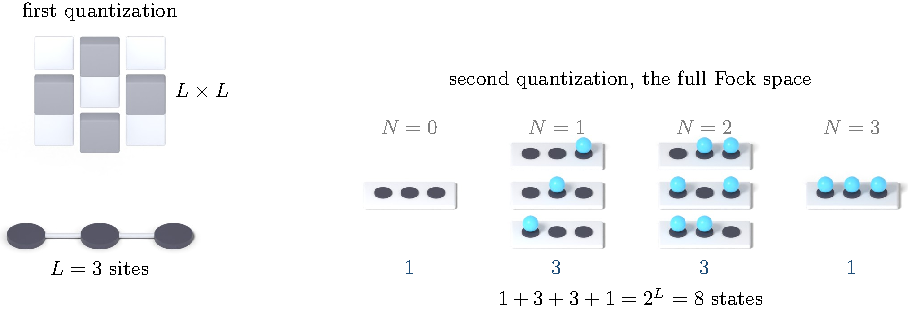
\includegraphics{figures/pdf/s01f01_fockspace.pdf}
\end{aqmfigure}


In general, for $L$ sites the single-particle problem is an $L \times L$ matrix, while the
many-body problem is a $2^L \times 2^L$ matrix, and we need $2^L$ coefficients only to write the
ground-state wave function. This is the reason why $L \approx 20$ is already close to the practical
limit of what we can do by brute force. The exact rate of growth depends on the kind of site that we
have. Spinful fermions have four states per site, which are empty, up, down and doubly occupied.
Spinless fermions have two, and they are relevant when a single spin species is isolated by strong
magnetism or a strong field. Pure spin sites, which we will need later in the course for quantum
magnets and Kondo systems, also give an exponential growth, but with a different underlying
algebra.

\section{A first look at eigenstates in finite tight-binding islands}

Before we go to interactions, let us look at what a purely single-particle Hamiltonian already gives
us, because this is something that we can compare directly with experiment. Let us take a
tight-binding Hamiltonian $H = \sum_{ij} t_{ij}\, c_i^\dagger c_j$ on a honeycomb lattice, cut into
a finite island that is triangular, hexagonal or rectangular, and let us diagonalize it. The
probability density of a given eigenvector in real space can be compared directly with what a
scanning tunneling microscope measures. Qualitatively, these states look like the finite-size
states of a ``particle in a box''. The lowest-energy state has its maximum close to the center of
the island, and the higher states have more and more nodes. This is a good first check, since
single-particle diagonalization, with nothing more, already gives a structure that we can recognize
and that we can measure in experiments.

\begin{notebookbox}{\texttt{session1.ipynb}, ``Finite sized chains'' (Core), and ``Density of states of a finite system as a function of the system size'' (Challenge)}
Diagonalize a finite chain or island, and look at how the spatial profiles of the eigenstates and
the density of states change when you make the system larger. This is the numerical version of the
particle-in-a-box argument above, and it is a good place to build intuition for how we approach an
infinite periodic system, which we treat in session 2, starting from the finite-size case.
\end{notebookbox}

We will use two software tools in all sessions. The first one is
\textbf{PyQula}, which is a Python library for tight-binding and mean-field calculations,
topological properties and spectral functions, and which we use through the Jupyter notebooks of
the course. The second one is \textbf{Quantum Lattice}, which is a graphical interface built on
PyQula that does not need any coding. Both are open source, and it is useful to have both open next
to these notes.

\section{Spontaneous symmetry breaking and why a symmetric Hamiltonian can have an asymmetric ground state}

Before we discuss interactions, let us ask a more general question, since everything that we do
in the rest of the session is an example of it. Physical theories usually have a lot of
symmetry. Space is symmetric, time is symmetric, and so on. However, reality is not symmetric,
since an object is in one place and not in another, and a system evolves forward in time and
usually not backward. So why do the symmetries of the Hamiltonian so often not survive in the
ground state?

Let us start with an example from daily life, which is a group of colleagues who sit at a
table for a meal, with bread on both sides of each person. Each person has to choose between the
bread on the left and the bread on the right. There is of course a ``correct'' answer from
etiquette, but let us say that nobody knows it. Some people will take the left one and others the
right one, and once the choice is made, everybody at the table ends up in one of two equally good
configurations, which are everybody-left or everybody-right. The initial setup, with bread on both
sides, was perfectly symmetric. The final result is not. This difference,
a symmetric problem with a solution that is not symmetric, is spontaneous symmetry breaking on a
small scale.

The same logic, in an exact form, is what happens in a classical Ising ferromagnet. The set of
ground states of the Hamiltonian is symmetric, since all spins up is as good a solution as all spins
down. However, if we take a \emph{very} large system, which formally means an infinitely large one,
or the thermodynamic limit, the system has to choose one of the two, all spins up or all spins down.
Which one we measure is decided by fluctuations and not by the Hamiltonian, and once it is decided,
the state that we observe is no longer symmetric, even though the Hamiltonian that produced it was
always symmetric. The requirement of the thermodynamic limit is essential. Strictly speaking,
spontaneous symmetry breaking is a statement about infinite systems, and it is a generic feature of
many-body interactions and correlations, not something that appears for a few particles.
Figure~\ref{fig:s01:ssb} puts all of this in one picture. It shows a symmetric energy landscape whose
minima are not symmetric, with a barrier between them that becomes impossible to cross only in the
thermodynamic limit.

% Session 1 -- spontaneous symmetry breaking: symmetric landscape, asymmetric minima.
% Placement: sec. "Spontaneous symmetry breaking", after the Ising paragraph.
% Rendered by figures/blender/s01f02_ssb.py, labels in figures/overlays/s01f02_ssb.tex.
\begin{aqmfigure}{fig:s01:ssb}{Spontaneous symmetry breaking. The energy as a function of the order
parameter is symmetric under $m\to-m$, in the same way as the Hamiltonian, but its minima are not,
since the system has to be at $+m_0$ or at $-m_0$. The system is the ball at $+m_0$, and the ghost
ball at $-m_0$ is the minimum with the same energy that it did not choose. The choice is made by
fluctuations and not by the Hamiltonian. The barrier between the minima grows with the system size,
from the small system on the left to the large one on the right, which is why spontaneous symmetry
breaking is strictly a statement about the thermodynamic limit.}
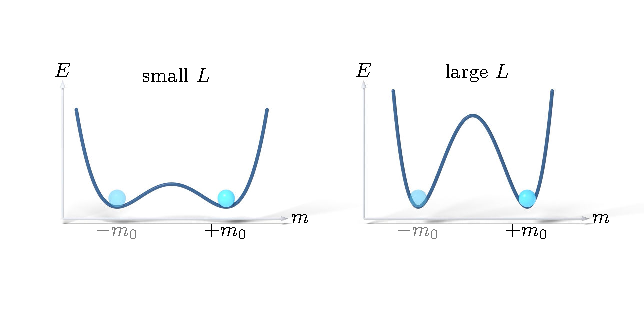
\includegraphics{figures/pdf/s01f02_ssb.pdf}
\end{aqmfigure}


This gives us a useful way to classify states of matter, according to \emph{which} symmetry they
break spontaneously.

\begin{itemize}
\item Broken \textbf{time-reversal symmetry} gives classical magnets. The magnetization is odd under
  time reversal, so a magnetic ground state is not invariant when we run the movie backward.
\item Broken \textbf{inversion symmetry} gives ferroelectrics. These are materials that
  develop an electric polarization spontaneously, which is the electric analog of a magnetization,
  and in this way they break the inversion symmetry of the underlying crystal.
\item Broken \textbf{gauge symmetry} gives superconductors. The phase of the pairing order
  parameter, or equivalently the phase of the creation and annihilation operators, becomes physical
  once the order appears. Many observable superconducting phenomena, such as the Josephson effect,
  are direct consequences of fluctuations of this broken phase, and we will discuss this in detail in
  the session on superconductivity.
\end{itemize}

This classification by symmetry is useful, but it does not capture everything. Topological materials, such as topological insulators and fractional Chern
insulators, can have \emph{exactly} the same broken or unbroken symmetries as an ordinary trivial
material and still behave in a completely different way. The reason for this is that they differ in
their topological classification and not in their symmetry classification. This difference is the
topic of a full session later in the course. For now, we only keep in mind that the question of
``which symmetry is broken'' does not give the full description of quantum matter.

Every case of spontaneous symmetry breaking also comes with its own emergent quasiparticle, which is
the low-energy fluctuation of the order that has formed. The following table lists three cases.

\begin{center}
\begin{tabular}{|l|l|l|c|c|l|}
\hline
\textbf{Broken symmetry} & \textbf{Realized in} & \textbf{Quasiparticle} & \textbf{Spin} & \textbf{Charge} & \textbf{Gap} \\
\hline
Continuous translational & Crystals & Phonon & 0 & 0 & Gapless (always) \\
Spin-rotational $SO(3)$ & Magnets & Magnon & 1 & 0 & Gapless (gapped with anisotropy) \\
Gauge & Superconductors & Higgs mode & 0 & 0 & Gapped \\
\hline
\end{tabular}
\end{center}

Note that magnons and the Higgs mode both have zero charge but very different spin, and that only
the phonon is gapless in every material. Magnons are gapless when the broken spin-rotational
symmetry is continuous, and they become gapped when a magnetic anisotropy breaks this symmetry
explicitly. The Higgs mode, which is an oscillation of the amplitude of the order parameter, is
always gapped.

Since we cannot run time backward in the lab to check if a material breaks time-reversal symmetry,
we measure instead quantities that are themselves odd under time reversal. Two of them are
especially useful. The first one is the \textbf{Hall conductivity}, which is a transverse current
generated by a longitudinal voltage. The second one is the \textbf{magneto-optical Kerr effect},
which is a different optical reflection for left-handed and right-handed circularly polarized light.
A nonzero signal in either of them is direct evidence of broken time-reversal symmetry.

With this we can finally give a precise and formal definition of a magnet, which goes beyond ``the
object that sticks to your fridge''. A magnet is a many-body state whose wave function is not
invariant under the time-reversal operator $\hat T$,

\begin{equation}
\hat T|\Psi\rangle = |\Psi\rangle \;\Rightarrow\; \text{not magnetic}, \qquad
\hat T|\Psi\rangle \neq |\Psi\rangle \;\Rightarrow\; \text{magnetic}.
\end{equation}

The north and south poles of a bar magnet are exchanged under time reversal, since a magnetic pole
is connected to an orbital angular momentum and angular momenta change sign under $\hat T$. For this
reason a bar magnet does not pass the invariance test in (1.4), and it is magnetic according to this
definition. A plain stick that is not magnetic, on the other hand, looks the same under time
reversal and passes the test.

Let us now build this general picture explicitly, three times.

\section{The general interacting Hamiltonian, and the tool we will use on it}

We can now state the problem that this whole session leads to. The Hamiltonians that we are
interested in have the generic form

\begin{equation}
H = \sum_{ij} t_{ij}\, c_i^\dagger c_j \;+\; \sum_{ijkl} V_{ijkl}\, c_i^\dagger c_j^\dagger c_k c_l,
\end{equation}

which is a free part, single-particle and exactly solvable, plus a quartic interaction. The
interaction itself can come from the plain electrostatic Coulomb repulsion, or from an effective
interaction mediated by some other quasiparticle, such as phonons, magnons or plasmons, which can
make the total interaction attractive instead of repulsive. We will treat these interactions in a
phenomenological way, as given effective models, and we will not derive them microscopically from
first principles.

To solve (1.5) exactly is in general impossible, for the exponential reason of Section 1.9.
\textbf{Mean-field theory} is the tool that still allows us to obtain systematic solutions from it,
even if they are approximate, and it can predict a wide range of symmetry-broken states. In this
session we will study three of them, which are the same three cases that we classified in Section
1.11.

\begin{enumerate}
\item \textbf{Broken time-reversal symmetry}, which is magnetism. If we run the movie of the system
   backward, it looks different from the original.
\item \textbf{Broken (lattice translational) symmetry}, which is the charge density wave. A
   Hamiltonian that is the same at every site at the start ends up with charge on some sites and
   not on others.
\item \textbf{Broken gauge symmetry}, which is superconductivity. The system develops an order
   parameter with a physical phase, which the symmetry of the original Hamiltonian does not allow.
\end{enumerate}

Figure~\ref{fig:s01:channels} shows these three branches next to each other, together with the
equation from which each one is developed and the session where it appears again.

% Session 1 -- one Hamiltonian, three broken symmetries.
% Placement: sec. "The general interacting Hamiltonian", alongside the enumerated list.
% Rendered by figures/blender/s01f03_threechannels.py, labels in figures/overlays/s01f03_threechannels.tex.
\begin{aqmfigure}{fig:s01:channels}{One Hamiltonian and three ordered states. The same generic
interacting Hamiltonian (1.5), on the left, where the glow is the interaction between two electrons
on neighboring sites, is decoupled with three different bilinear expectation values. This gives a
charge density wave, a magnet or a superconductor, each breaking a different symmetry. The charge is
drawn as columns of alternating height, the spin as alternating arrows, and the electrons bound in
pairs as two balls inside one capsule. These three branches are the structure on which the rest of
the course is organized.}
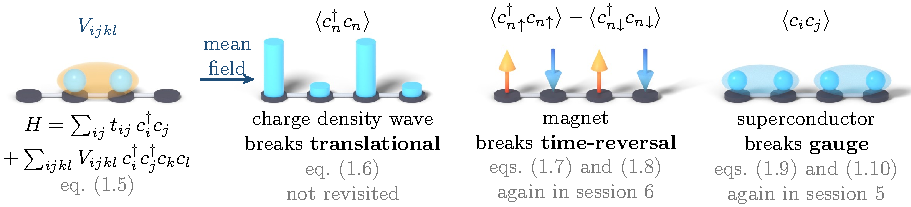
\includegraphics{figures/pdf/s01f03_threechannels.pdf}
\end{aqmfigure}


Two of the three cases of this session, which are magnetism and superconductivity, will come back
later in the course in their own sessions, where we treat them in much more detail. You can think of
what follows as a first pass, whose goal is to set up the mean-field method itself, and not as the
final discussion of either of them.

\section{Worked example 1, the charge density wave}

Let us take the simplest interacting case, which is a spinless one-dimensional chain with
nearest-neighbor hopping $t$ and a nearest-neighbor Coulomb repulsion $V$,

\begin{equation}
H = -t\sum_n \left(c_n^\dagger c_{n+1} + \text{h.c.}\right) + V\sum_n c_n^\dagger c_n\, c_{n+1}^\dagger c_{n+1}.
\end{equation}

In this form, every site is equivalent because of translational symmetry. The quartic term is the
difficult one, so mean-field theory factorizes it. We replace one pair of operators by its
expectation value, and we keep the rest as it is. This is an \emph{uncontrolled} approximation, and
a more rigorous way exists with a path integral and a saddle-point approximation, but it is the
practical method that we will use in the whole course. As a result, the interaction term becomes a
single-particle onsite energy that depends on the position. Nothing forces the expectation value
$\langle c_n^\dagger c_n\rangle$ to be the same at every site, so even if the bare Hamiltonian (1.6)
is translationally symmetric, the mean-field solution does not have to be. This difference, a
symmetric Hamiltonian with an asymmetric ground state, \emph{is} the charge density wave, and it is
the same difference that Section 1.11 described in the abstract.

More rigorously, mean-field theory is a variational search over single-particle product
states, where we minimize $\langle H\rangle$ with respect to the bilinear expectation values $\langle
c_i^\dagger c_j\rangle$ that define the mean-field Hamiltonian. Since the Hamiltonian depends on
these expectation values and the expectation values depend on the Hamiltonian, we solve the problem
self-consistently. We guess a Hamiltonian, we compute the expectation values that it gives, we build
a new Hamiltonian from them, and we repeat until the process converges. Figure~\ref{fig:s01:mfloop}
shows this loop, and every worked example below and every notebook box in this chapter uses it.

% Session 1 -- the mean-field self-consistency loop.
% Placement: sec. "Worked example 1", at the "more rigorously, mean-field theory is a
% variational search..." paragraph.
% Rendered by figures/blender/s01f05_selfconsistency.py, labels in figures/overlays/s01f05_selfconsistency.tex.
\begin{aqmfigure}{fig:s01:mfloop}{The mean-field self-consistency loop. We guess the bilinear
expectation values, build the single-particle Hamiltonian that they give, and diagonalize it. Then
we compute the new expectation values and repeat until they do not change anymore. The four stations
are one pass of the loop, computed for the charge density wave of (1.6) on a periodic chain of four
sites with $V=3t$. The guessed charges $0.6$ and $0.4$, drawn as columns, raise the onsite energy of
the neighboring sites, so the sites of the mean-field Hamiltonian stand at two heights. Filling its
two lowest levels gives the new charges $0.82$ and $0.18$, which are not the guess, so the loop goes
round again. The three worked examples of this session and every notebook box in this chapter use
this same loop.}
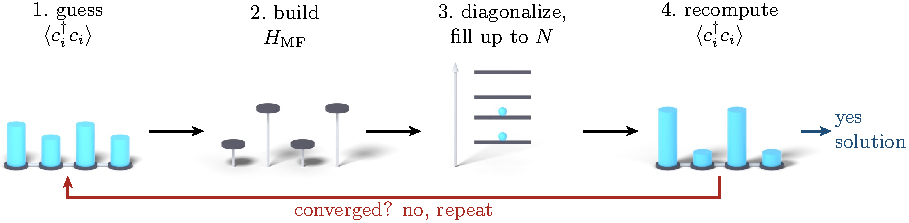
\includegraphics{figures/pdf/s01f05_selfconsistency.pdf}
\end{aqmfigure}


Numerically, at $V=0$ the spectrum is gapless, which is a metal. When $V$
grows, a gap opens in the single-particle spectrum and becomes larger, and at the same time the
charge imbalance between even and odd sites grows from zero toward its maximal value, where it is
fully polarized. Figure~\ref{fig:s01:cdw} shows the two limits in real space, together with the
spectrum of each one.

% Session 1 -- the charge density wave in real space.
% Placement: sec. "Worked example 1", at the "numerically, this shows up..." paragraph.
% Rendered by figures/blender/s01f04_cdw.py, labels in figures/overlays/s01f04_cdw.tex.
\begin{aqmfigure}{fig:s01:cdw}{The charge density wave of the chain (1.6), solved in mean field for
a periodic chain of eight sites at half filling. The height of the liquid in each cup is the charge
$\langle n_i\rangle$, and next to each chain is its single-particle spectrum, with an electron on
every occupied level and degenerate levels side by side. In front, at $V=0$, every site has the same
charge and the spectrum is gapless, since the Fermi level is inside a pair of degenerate levels.
Behind, the nearest-neighbor repulsion drives the mean-field instability (here $V=3t$), and the
charge accumulates on alternating sites, which doubles the unit cell, drawn as the translucent slab,
and opens a gap in the spectrum. The Hamiltonian is translationally symmetric in both cases, but the
ground state behind is not.}
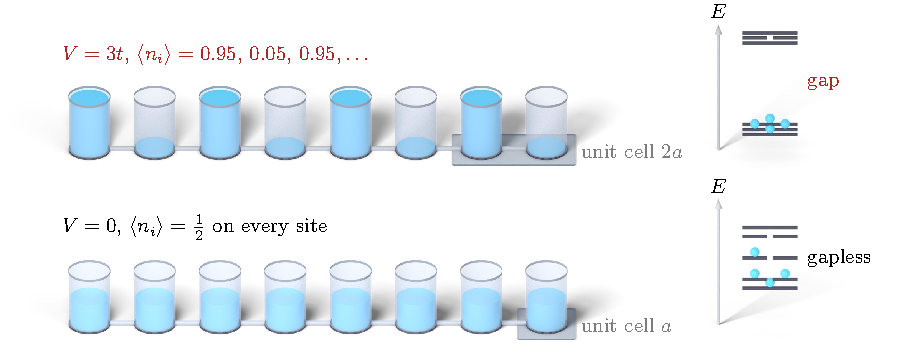
\includegraphics{figures/pdf/s01f04_cdw.pdf}
\end{aqmfigure}


\begin{notebookbox}{\texttt{session1.ipynb}, ``Symmetry breaking in the spinless fermionic chain'' (Core), and ``Gap opening in a spinless interacting model'' (Challenge)}
Run the self-consistency loop of Section 1.13 yourself. Start from an unbiased guess, iterate, and
look at how the charge imbalance on each site grows with $V$, together with the opening of the gap
in the spectrum and in the density of states.
\end{notebookbox}

\section{Worked example 2, magnetism}

Let us now include again the spin degree of freedom, and let us change the interaction to an onsite
Hubbard term between spin-up and spin-down electrons,

\begin{equation}
H = -t\sum_{n,\sigma}\left(c_{n\sigma}^\dagger c_{n+1,\sigma} + \text{h.c.}\right) + U\sum_n c_{n\uparrow}^\dagger c_{n\uparrow}\, c_{n\downarrow}^\dagger c_{n\downarrow}.
\end{equation}

The sign of $U$ alone decides the physics. An attractive $U<0$ drives superconductivity, which we
discuss in Section 1.15, and a repulsive $U>0$ drives magnetism, which is the topic of this section.

The mean-field decoupling is done in the same way as before, but now we apply it separately to
$\langle c_{\uparrow}^\dagger c_\uparrow\rangle$ and $\langle c_\downarrow^\dagger
c_\downarrow\rangle$, and we obtain a bilinear Hamiltonian with onsite energies that depend on the
spin. Let us define the magnetization

\begin{equation}
m = \langle c_\uparrow^\dagger c_\uparrow\rangle - \langle c_\downarrow^\dagger c_\downarrow\rangle.
\end{equation}

Self-consistency gives $m=0$ automatically for $U<0$, and a finite $m$ for $U>0$, which is a real
magnetic solution.

Let us say precisely \emph{which} symmetry is broken here, using the formal definition in (1.4).
Time-reversal symmetry reverses the direction of time and, together with it, every angular momentum
in the system, including the spin. On the fermionic operators this means that it exchanges
$c_\uparrow^\dagger c_\uparrow \leftrightarrow c_\downarrow^\dagger c_\downarrow$. Since $m$ in
(1.8) changes sign under this exchange, a nonzero $m$ means that the ground state does not pass the
invariance test in (1.4), so it is a magnet by definition. More generally, this is a breaking of the
\emph{continuous} spin-rotational symmetry, and this continuous symmetry breaking is what gives rise
to the gapless magnon excitations that appear in the table of Section 1.11. We will study them in
detail in a later session, and in this session we only need the mean-field ground state itself.

Numerically, when we increase $U$ a \textbf{Mott gap} opens in the spectrum, which grows linearly
with $U$ at large $U$ and is associated with the formation of a real local moment on every site.

\begin{notebookbox}{\texttt{session1.ipynb}, ``The interacting Hubbard dimer'' (Core), ``Magnetic order driven by interactions in a chain'' (Core), ``Gap opening of the Hubbard model in a chain'' (Challenge), and ``Gap opening in the Hubbard model on the honeycomb lattice'' (Challenge)}
Start with the two-site case, the dimer, to see how the self-consistency loop converges in a small
system that you can check by hand. Then go to the extended chain and finally to the honeycomb
lattice, which uses the same finite-island geometries of Section 1.10 but now with interactions, and
look at how the Mott gap opens and grows with $U$.
\end{notebookbox}

\section{Worked example 3, superconductivity and broken gauge symmetry}

Let us go back to (1.7) with $U<0$. The mean-field decoupling that we used above always keeps one
creation operator and one annihilation operator together, but nothing forces this choice. We can
also take an expectation value of two creation operators, or of two annihilation operators,

\begin{equation}
\Delta = \langle c_i c_j\rangle.
\end{equation}

This anomalous term, which is called a ``pairing'' term, looks qualitatively different from all the
terms that we wrote so far, but it is a valid mean-field term. In the self-consistent solution,
$\Delta$ is zero for repulsive interactions and can become nonzero for attractive ones, and this is
the superconducting order parameter. This worked example is only in the slides, and there is no
notebook section for it in this session. The pairing formalism, which is the Bogoliubov-de Gennes
formalism that we need to solve it numerically, is left for the session on superconductivity.

Why does this order break gauge symmetry? A gauge transformation acts on the operators as

\begin{equation}
c \to c\, e^{i\varphi}, \qquad c^\dagger \to c^\dagger e^{-i\varphi}.
\end{equation}

Any term built from one creation operator and one annihilation operator, $c^\dagger c$, is invariant
under (1.10), since the two phases cancel. However, the pairing term in (1.9) is built from
\emph{two} annihilation operators, or two creation operators, so under the same transformation it
gets a phase $e^{2i\varphi}$, or $e^{-2i\varphi}$, which does not cancel. For this reason a
superconductor with $\Delta \neq 0$ breaks the gauge symmetry of the Hamiltonian spontaneously, which
is the ``broken gauge symmetry'' case in the classification of Section 1.11. This is directly
connected to the puzzle of Section 1.5 about a fluctuating number of electrons. To break gauge
symmetry and to lose a fixed number of particles are, physically, the same statement. A mean-field
superconductor does not have a fixed number of electrons, only a fixed parity.

\section{Closing summary}

\begin{itemize}
\item Quantum materials realize a very large range of phenomena, such as topological order,
  fractionalization and correlated superconductivity, that no single atom shows on its own. The
  central question of this course is to understand how these phenomena emerge from electrons in a
  lattice.
\item \textbf{Second quantization} is the language that allows us to treat in the same way systems
  with a fixed number of particles, which are single-particle systems, and systems with a
  fluctuating number of particles, which are many-body systems. It is built from creation and
  annihilation operators that satisfy the anticommutation relations (1.3).
\item The many-body Hilbert space grows as $2^L$, as we saw in Section 1.9, and for this reason
  interacting problems need a systematic approximation and not brute-force diagonalization.
\item \textbf{Spontaneous symmetry breaking} is the general phenomenon where a symmetric Hamiltonian
  gives an asymmetric ground state in the thermodynamic limit. We can classify states of matter by
  the symmetry that they break, which is time-reversal for magnets, inversion for ferroelectrics
  and gauge for superconductors, and each case has its own emergent quasiparticle. A magnet has the
  precise and formal definition given in (1.4). Topological materials show that this
  classification does not cover all cases.
\item \textbf{Mean-field theory} gives the practical method. We factorize the interacting
  Hamiltonian (1.5) by taking an expectation value of part of the quartic term, and then we solve
  the resulting single-particle problem self-consistently.
\item The same procedure, applied to three different interaction channels, gives three different
  symmetry-broken states. These are a charge density wave from (1.6), with broken translational
  symmetry, a magnet from (1.7)-(1.8), with broken time-reversal symmetry, and a superconductor from
  (1.9)-(1.10), with broken gauge symmetry. Magnetism and superconductivity each have a full session
  later in the course, and the versions of this session are a first pass.
\end{itemize}

In the next session we leave interactions aside for some time, and we go back to the
single-particle part of the Hamiltonian of this session. We will see how \emph{symmetry}, and in
particular translational symmetry, allows us to diagonalize it exactly, without any approximation,
using Bloch's theorem. The general framework of symmetry breaking that we built in Section 1.11 will
not be discussed again there, so it is useful to keep it from here and not to expect a summary of
it later.
